% !TeX root = ../main.tex
\chapter{测量平台设计与搭建}



\section{总体设计}\label{sec:rig-overall}

根据上文规划的测量方案以及实际需求,设计大气环境下的静电卡盘静电力检测平台,希望能达成如下目标:

\begin{enumerate}
  \item 实现用背吹平衡 -- 微力探头法检测静电力
  \item 自动化检测过程,减小人为误差
  \item 采集检测过程中各关键变量,方便后续数据处理与分析
\end{enumerate}

下面将详细阐述测量平台的设计方案。


\subsection{测量平台组成}\label{sec:rig-overall-comp}

\begin{figure}[tbh]
\centering
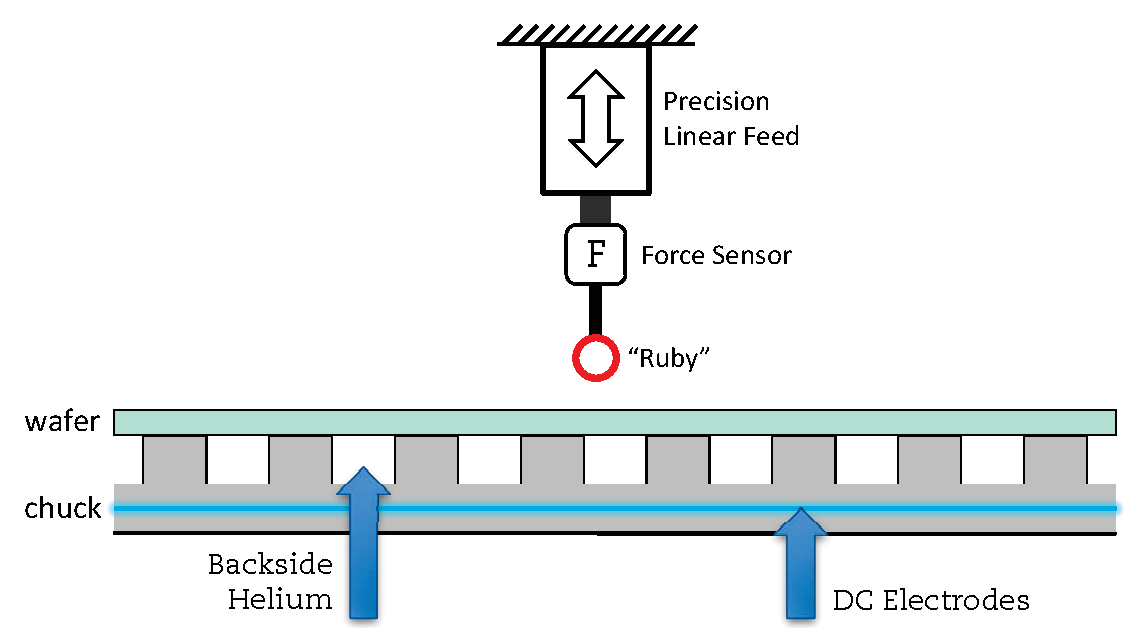
\includegraphics[width=1\linewidth]{rig/sch}
\caption{测量平台总体设计示意}
\label{fig:rig-sch}
\end{figure}

如图~\ref{fig:rig-sch},整个测量平台由以下组件构成:

\begin{itemize}
  \item 待测静电卡盘及其配套静电电源
  \item 微力探头组件
  \item 背吹控制系统
  \item 机械结构
  \item 电子总控与数据采集系统
\end{itemize}

除静电卡盘与电源外,其他组件均需自行设计、搭建。


\subsection{检测流程}

一次完整的检测过程分如下步骤完成:

\begin{enumerate}
  \item 准备静电卡盘
  \begin{enumerate}
    \item 用无水乙醇擦拭静电卡盘与晶圆
    \item 将晶圆小心地放置在静电卡盘陶瓷层正中央
    \item 开启静电电源,调节电极电压至目标电压
  \end{enumerate}
  
  \item 准备测量平台
  \begin{enumerate}
    \item 降下微力探头,使其轻轻接触晶圆
    \item 确认背吹控制系统中调压装置均处于零位
  \end{enumerate}
  
  \item 检测
  \begin{enumerate}
    \item 开始自动记录微力探头受力、背吹入口气压两变量
    \item 背吹气压接通并缓慢、均匀地上升
    \item 当微力探头受力即将达到其满量程时,自动切断背吹气压,检测停止
  \end{enumerate}
  
  \item 后续处理
  \begin{enumerate}
    \item 导出采集到的数据
    \item 微力探头复位上升
    \item 切断静电电源,短接两电极引线,消除部分残余电荷
    \item 小心将晶圆取下
  \end{enumerate}
\end{enumerate}



\section{微力探头组件设计}\label{sec:rig-probe}

图~\ref{fig:rig-sch}中,卡盘上方的组件即为微力探头组件微力探头组件,其在\ref{principle-gap-ruby}一节中提到的微力传感器和红宝石探头的基础上,增设精密直线进给机构:固定端连接在框架上,移动端与力传感器的固定端相连,用于驱动探头沿z方向移动,以实现“轻轻接触晶圆”这一动作。


\subsection{微力传感器选型}

微力传感器是探头组件中的核心元件,其性能直接关系到探头能否正常发挥作用,因此优先选型。考虑到其在测量系统中的作用,需重点考察的指标如下:

\begin{enumerate}
  \item
    量程:无论在轻触阶段还是在脱附检测阶段,探头均不应向晶圆施加过大的力。粗估静电力处于$\SI{10}{\newton}$至$\SI{200}{\newton}$之间,探头施加的力应低于其$1 ~\%$,即微力传感器应能准确测量 大致在$\SI{0.1}{\newton}$至$\SI{2}{\newton}$范围内的单轴压缩力。
  \item
    分辨力:微力传感器需能检测到微小的受力变化,根据上述关于量程的讨论,应能至少分辨出$\SI{1}{\micro\newton}$的力增量。不同的传感器可能对分辨力的标称方法不同,应结合其输出信号特点,判定其是否满足要求。
  \item
    刚度:微力传感器的敏感端存在一位移,一般服从胡克定律,与受力成比例关系。\ref{principle-gap}一节中讨论了晶圆与卡盘间气隙可能对静电力产生的影响。
  \item
    过载能力:考虑到在安装、调试过程中,以及硅晶圆突然完全脱附时,探头均可能瞬间受到较大的力的作用;若微力传感器承受过载能力较好,则可避免其意外受损。
\end{enumerate}

市面上常见的微力传感器主要有应变式、压电式两种,其他类型的还有MEMS式等。经初步筛选,将以下产品作为备选方案:

%TODO:sensor table







\section{背吹控制回路设计}\label{sec:rig-pressure}

%TODO: update pressure schematic
\begin{figure}[tbh]
\centering
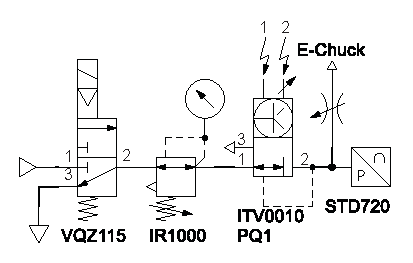
\includegraphics[width=0.618\linewidth]{rig/pressure__sch__full}
\caption{整体气路图}
\label{fig:rig-pressure-sch-full}
\end{figure}



\section{机械结构设计}\label{sec:rig-model}

\begin{figure}[p]
\centering
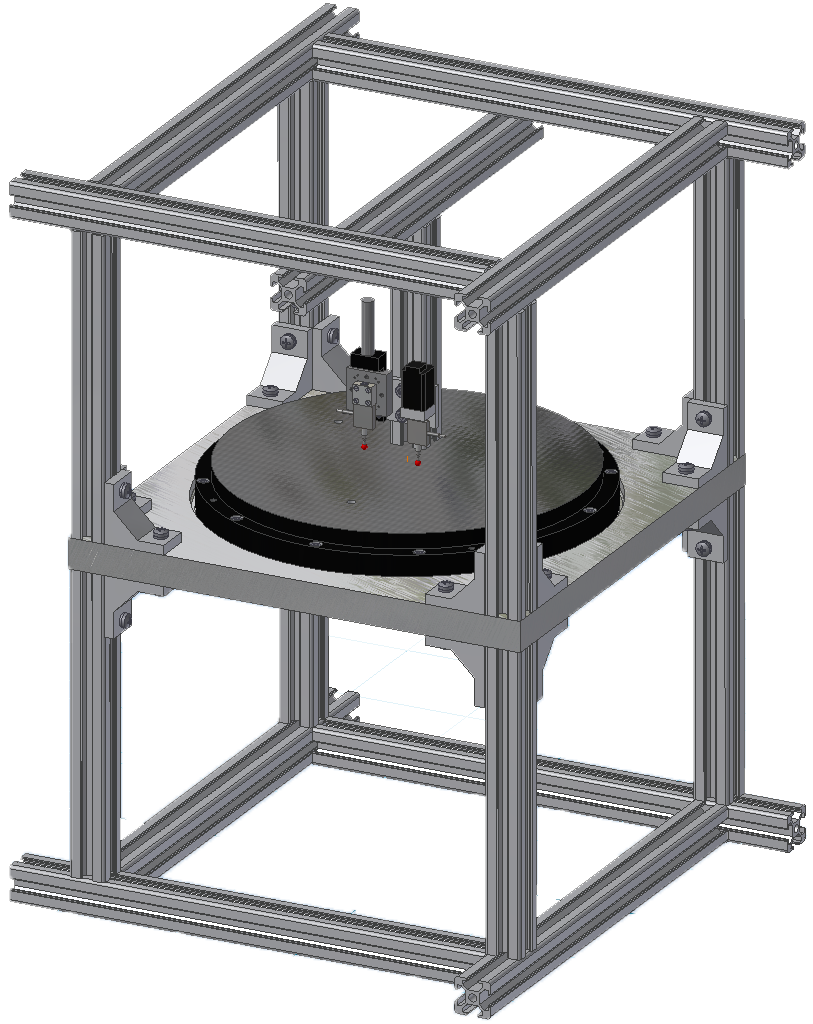
\includegraphics[width=1\textwidth]{rig/model__all__iso.png}
\caption{试验台整体数字模型}
\label{fig:rig-model-all-iso}
\end{figure}

\begin{figure}[tbhp]
\centering
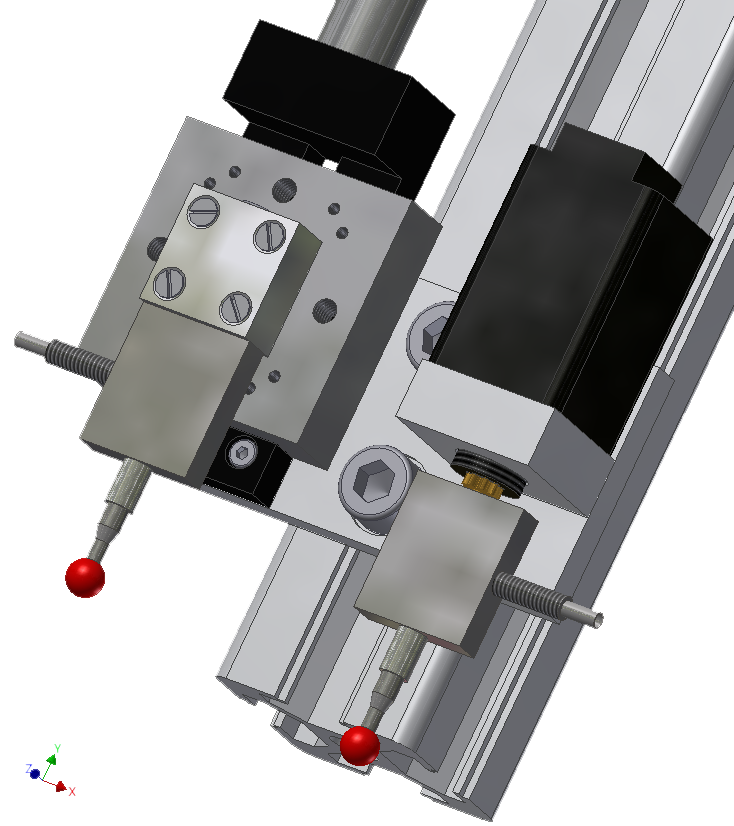
\includegraphics[height=0.45\textheight]{rig/model__probe.png}
\caption{探头组件数字模型}
\label{fig:rig-model-probe}
\end{figure}


